\chapter{Experiment Results and conclusion}
\label{expt}
\section{Part A: Object Recognition of the CIFAR-10 dataset}
\label{part1}

The details of this dataset are as follows:
\begin{quote}
The dataset contains RGB colour images of size 32 X 32 and their labels from 0 to 9. You will be using the batch-1 of the dataset, which contains 10,000 training samples. Testing is done on 2,000 test samples. The training data and testing data are provided in files 'data\_batch\_1' and 'test\_batch\_trim' files, respectively. Sample code is given in file start\_project\_2a.py Design a convolutional neural network consisting of:

\begin{itemize}
    \item An Input layer of 3x32x32 dimensions
    \item A convolution layer $C_1$ of 50 filters of window size 9x9, VALID padding, and ReLU neurons. A max pooling layer $S_1$ with a pooling window of size 2x2, with stride = 2 and padding = 'VALID'.
    \item A convolution layer $C_2$ of 60 filters of window size 5x5, VALID padding, and ReLU neurons. A max pooling layer $S_2$ with a pooling window of size 2x2, with stride = 2 and padding = 'VALID'.
    \item A fully connected layer $F_3$ of size 300.
    \item A softmax layer $F_4$ of size 10.
\end{itemize}
\end{quote}

The definition of the cnn network as required by the question is shown in Listing \ref{ls:1_l3}, whereas the loss minimisation and accuracy prediction is shown in Listing \ref{ls:1_loss}.

\begin{lstlisting}[language=Python, caption= Definition of the cnn network, label=ls:1_l3]
def cnn(images, num_filter_1, num_filter_2, dropout=False):
    # NHWC format
    images = tf.reshape(images, [-1, IMG_SIZE, IMG_SIZE, NUM_CHANNELS])
    
    #Conv 1, 50 filters of window size 9x9, VALID padding, and ReLU
    with tf.variable_scope('CNN_Layer1'):
        conv1 = tf.layers.conv2d(
            images,
            filters=num_filter_1,
            kernel_size=[9,9],
            padding='VALID',
            activation=tf.nn.relu)
        pool1 = tf.layers.max_pooling2d(
            conv1,
            pool_size=2,
            strides=2,
            padding='VALID')
        if dropout:
            pool1 = tf.layers.dropout(pool1, 0.25)

    with tf.variable_scope('Char_CNN_Layer2'):
        conv2 = tf.layers.conv2d(
            pool1,
            filters=num_filter_2,
            kernel_size=[5,5],
            padding='VALID',
            activation=tf.nn.relu)
        pool2 = tf.layers.max_pooling2d(
            conv2,
            pool_size=2,
            strides=2,
            padding='VALID')
        if dropout:
            pool2 = tf.layers.dropout(pool2, 0.25)

    dim = pool2.get_shape()[1].value * pool2.get_shape()[2].value * pool2.get_shape()[3].value 
    pool2_ = tf.reshape(pool2, [-1, dim])
    
    # Fully connected layer size 300
    f3 = tf.layers.dense(pool2_, 300, activation=tf.nn.relu)
    if dropout:
        f3 = tf.layers.dropout(f3, 0.5)

    #Softmax, size 10. Note that softmax happens at softmax_entropy step
    f4 = tf.layers.dense(f3, NUM_CLASSES, activation=None)

    return conv1, pool1, conv2, pool2, f4
\end{lstlisting}

\begin{lstlisting}[language=Python, caption= Loss minimisation and accuracy prediction, label=ls:1_loss]
x = tf.placeholder(tf.float32, [None, IMG_SIZE*IMG_SIZE*NUM_CHANNELS])
y_ = tf.placeholder(tf.float32, [None, NUM_CLASSES])

conv_1, pool_1, conv_2, pool_2, logits = cnn(x, 50, 60)
cross_entropy = tf.nn.softmax_cross_entropy_with_logits_v2(labels=y_, logits=logits)
loss = tf.reduce_mean(cross_entropy)
train_step = tf.train.GradientDescentOptimizer(learning_rate).minimize(loss)

correct_prediction = tf.equal(tf.argmax(logits, 1), tf.argmax(y_, 1))
correct_prediction = tf.cast(correct_prediction, tf.float32)
accuracy = tf.reduce_mean(correct_prediction)
\end{lstlisting}

Additionally the handling of batches sizes are shown in Listing \ref{ls:1_batch_size}.

\begin{lstlisting}[language=Python, caption= Batch size setup, label=ls:1_batch_size]
# Handle in batches
for start, end in zip(range(0, len(train_X), batch_size), range(batch_size, len(train_X), batch_size)):
    _, batch_cost = sess.run([train_step, loss], {x: train_X[start:end], y_: train_Y[start:end]})
    train_cost_.append(batch_cost)
\end{lstlisting}

Finally, the training results used in this experiment is assumed to be the ones obtained from cross-validation obtained from Listing \ref{ls:1_folds}, while the test set used are assumed to be the test set obtained from the initial 70:30 split from the original data.

\subsection{Question 1}
\label{1q1}
\begin{quote}
Train the network by using mini-batch gradient descent learning. Set $batch size =128$, and learning rate $\alpha = 0.001$. Images should be scaled.

a. Plot the training cost and the test accuracy against learning epochs.

b. For any two test patterns, plot the feature maps at both convolution layers ($C_1$ and $C_2$) and pooling layers ($S_1$ and $S_2$) along with the test patterns.
\end{quote}

\subsubsection{Part A}
The following plot in Figure \ref{fig:1a} is obtained for Q1a.
\begin{figure}[H]
    \begin{subfigure}{1\textwidth}
        \centering
        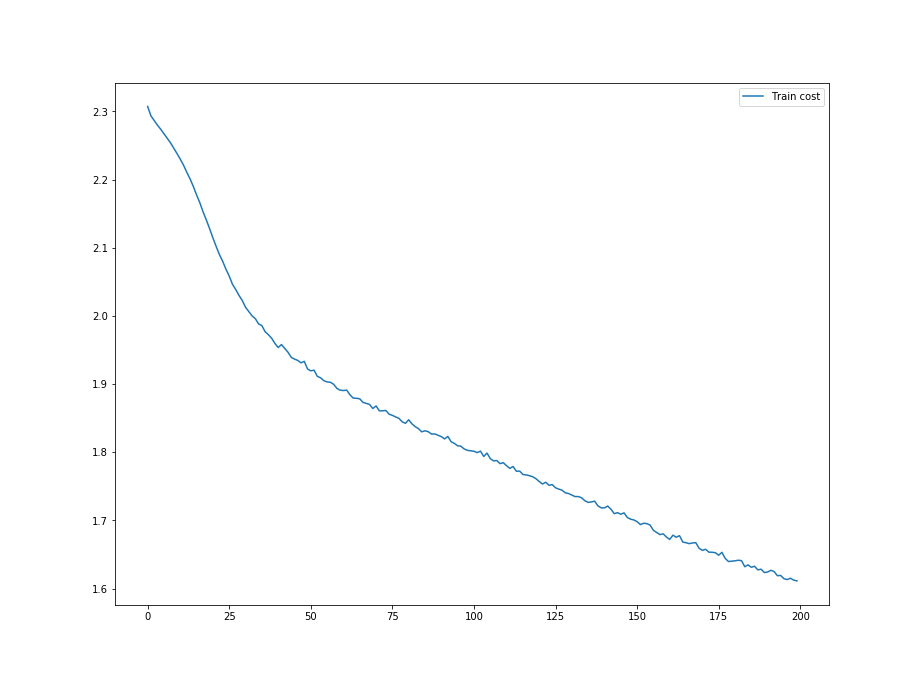
\includegraphics[width=0.8\linewidth]{assets/plots1/q1a_1.png}
        \caption{Training cost against epochs for cnn}
    \end{subfigure}
    \begin{subfigure}{1\textwidth}
        \centering
        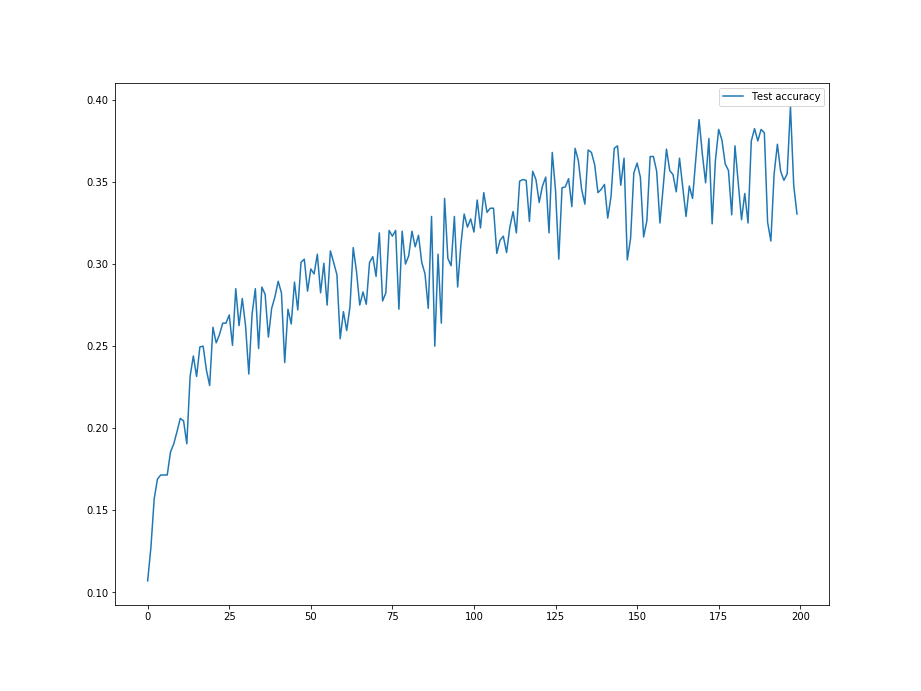
\includegraphics[width=0.8\linewidth]{assets/plots1/q1a_2.png}
        \caption{Test accuracy against epochs for cnn}
    \end{subfigure}
    \caption{Plot of training cost and testing accuracy against epochs for CNN object recognition}
    \label{fig:1a}
\end{figure}

\subsubsection{Part B}
Test Pattern 1 is shown in Figure \ref{fig:1b_1}.
\begin{figure}[H]
    \begin{subfigure}{0.5\textwidth}
        \centering
        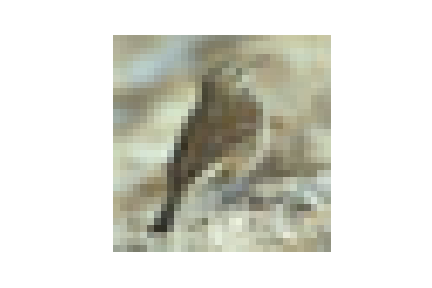
\includegraphics[width=1\linewidth]{assets/plots1/q1a_test_pattern_0.png}
        \caption{Test Pattern}
    \end{subfigure}
    \begin{subfigure}{0.5\textwidth}
        \centering
        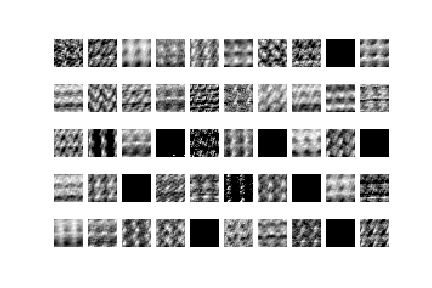
\includegraphics[width=1\linewidth]{assets/plots1/q1a_conv1_0.png}
        \caption{$\textit{C}_1$ Feature Map}
    \end{subfigure}
    \begin{subfigure}{0.5\textwidth}
        \centering
        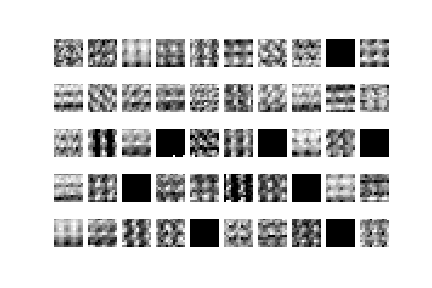
\includegraphics[width=1\linewidth]{assets/plots1/q1a_pool1_0.png}
        \caption{$\textit{S}_1$ Feature Map}
    \end{subfigure}
    \begin{subfigure}{0.5\textwidth}
        \centering
        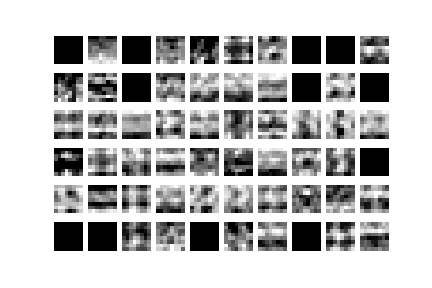
\includegraphics[width=1\linewidth]{assets/plots1/q1a_conv2_0.png}
        \caption{$\textit{C}_2$ Feature Map}
    \end{subfigure}
    \begin{subfigure}{0.5\textwidth}
        \centering
        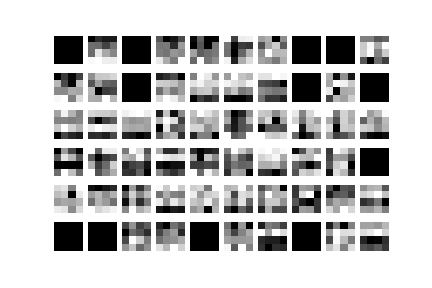
\includegraphics[width=1\linewidth]{assets/plots1/q1a_pool2_0.png}
        \caption{$\textit{S}_2$ Feature Map}
    \end{subfigure}
    \caption{Feature maps of test pattern 1}
    \label{fig:1b_1}
\end{figure}

Test Pattern 2 is shown in Figure \ref{fig:1b_2}.
\begin{figure}[H]
    \begin{subfigure}{0.5\textwidth}
        \centering
        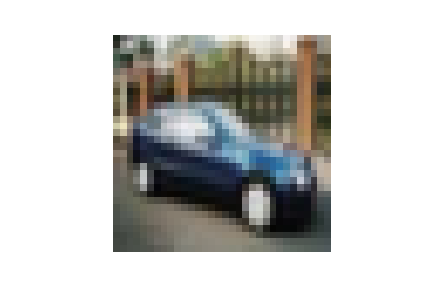
\includegraphics[width=1\linewidth]{assets/plots1/q1a_test_pattern_1.png}
        \caption{Test Pattern}
    \end{subfigure}
    \begin{subfigure}{0.5\textwidth}
        \centering
        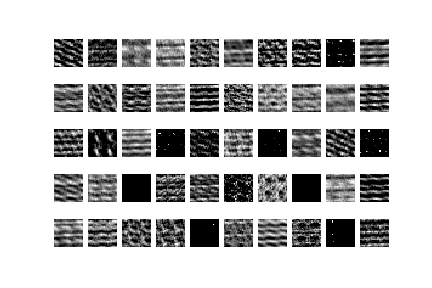
\includegraphics[width=1\linewidth]{assets/plots1/q1a_conv1_1.png}
        \caption{$\textit{C}_1$ Feature Map}
    \end{subfigure}
    \begin{subfigure}{0.5\textwidth}
        \centering
        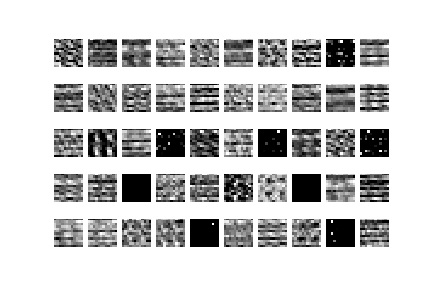
\includegraphics[width=1\linewidth]{assets/plots1/q1a_pool1_1.png}
        \caption{$\textit{S}_1$ Feature Map}
    \end{subfigure}
    \begin{subfigure}{0.5\textwidth}
        \centering
        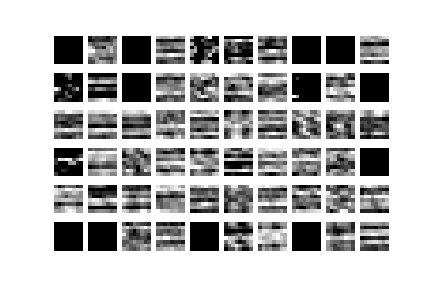
\includegraphics[width=1\linewidth]{assets/plots1/q1a_conv2_1.png}
        \caption{$\textit{C}_2$ Feature Map}
    \end{subfigure}
    \begin{subfigure}{0.5\textwidth}
        \centering
        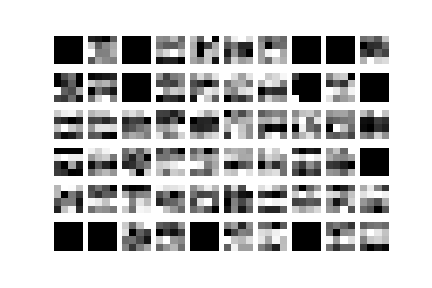
\includegraphics[width=1\linewidth]{assets/plots1/q1a_pool2_1.png}
        \caption{$\textit{S}_2$ Feature Map}
    \end{subfigure}
    \caption{Feature maps of test pattern 2}
    \label{fig:1b_2}
\end{figure}

\subsection{Question 2}
\label{1q2}
\begin{quote}
Using a grid search, find the optimal numbers of feature maps for part (1) at the convolution layers. Use the test accuracy to determine the optimal number of feature maps.
\end{quote}

\subsubsection{Part A}
\begin{figure}[H]
    \begin{subfigure}{0.5\textwidth}
        \centering
        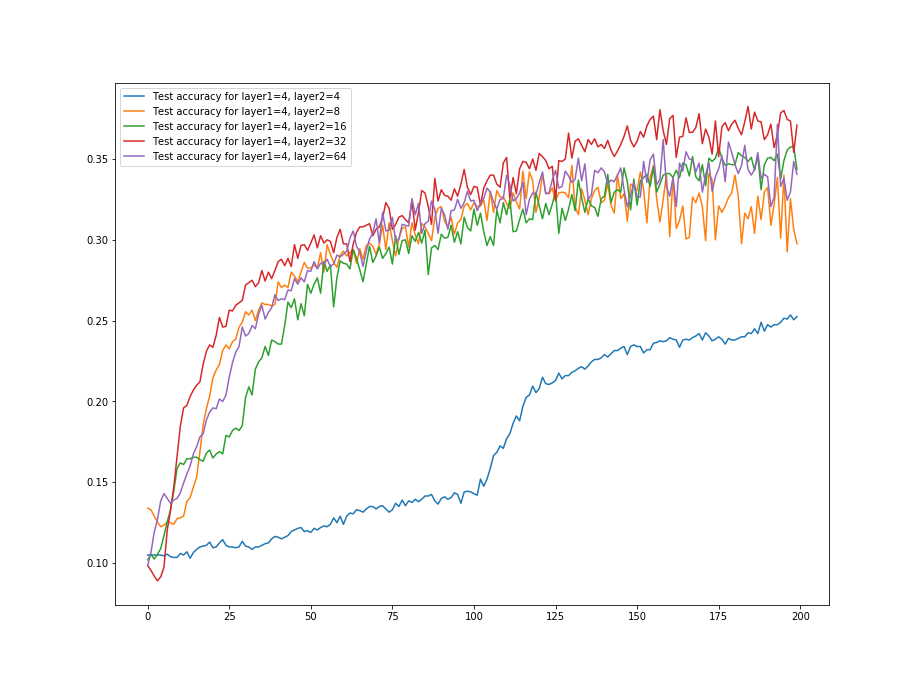
\includegraphics[width=1\linewidth]{assets/plots1/q2_0.png}
        \caption{Training cost for cnn}
    \end{subfigure}
    \begin{subfigure}{0.5\textwidth}
        \centering
        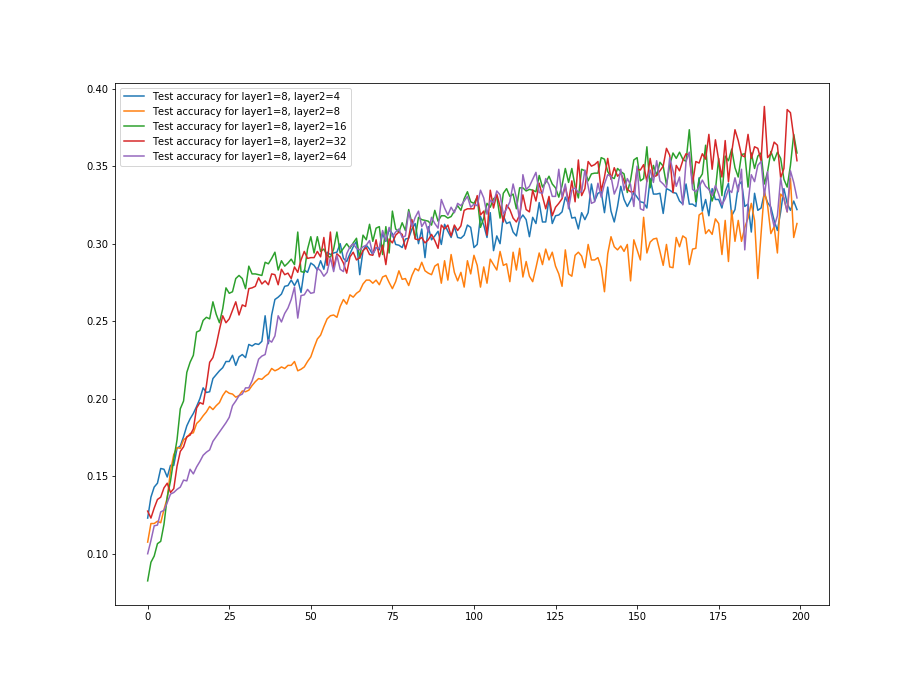
\includegraphics[width=1\linewidth]{assets/plots1/q2_1.png}
        \caption{Training cost for cnn}
    \end{subfigure}
    \begin{subfigure}{0.5\textwidth}
        \centering
        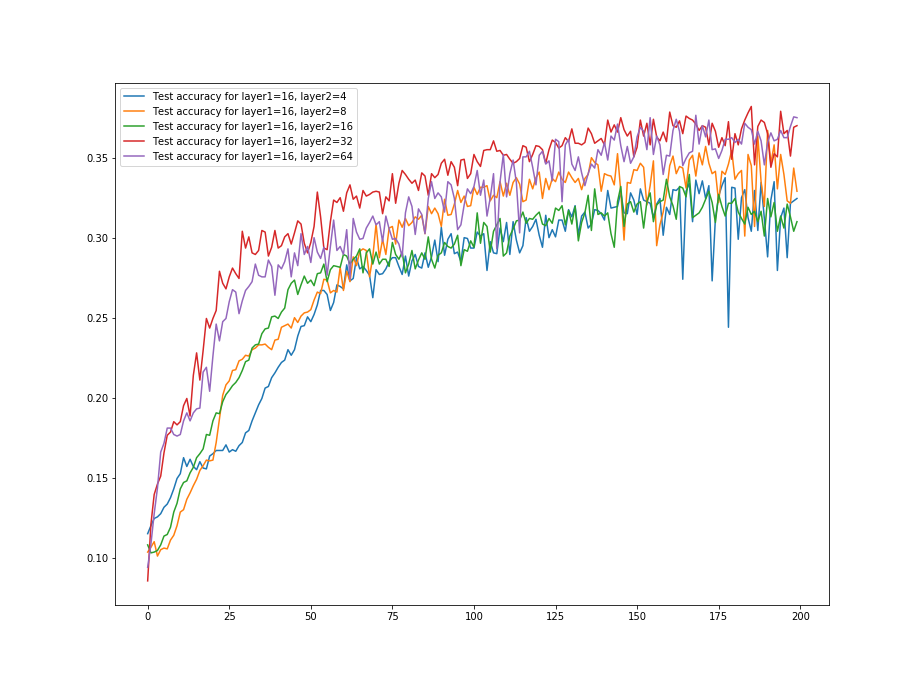
\includegraphics[width=1\linewidth]{assets/plots1/q2_2.png}
        \caption{Test accuracy for cnn}
    \end{subfigure}
    \begin{subfigure}{0.5\textwidth}
        \centering
        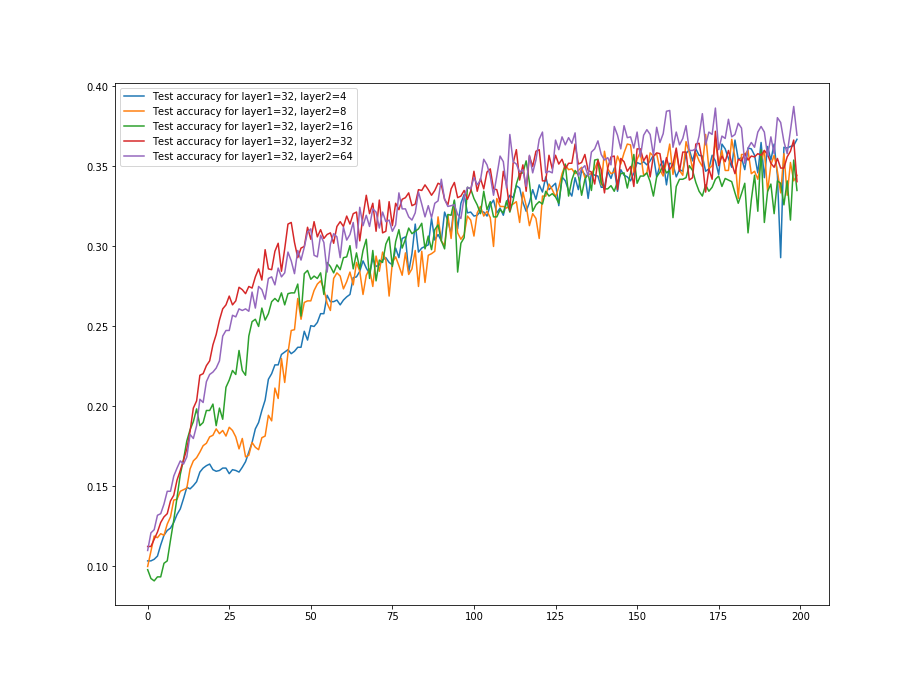
\includegraphics[width=1\linewidth]{assets/plots1/q2_3.png}
        \caption{Test accuracy for cnn}
        \label{fig:2_4}
    \end{subfigure}
    \begin{subfigure}{0.5\textwidth}
        \centering
        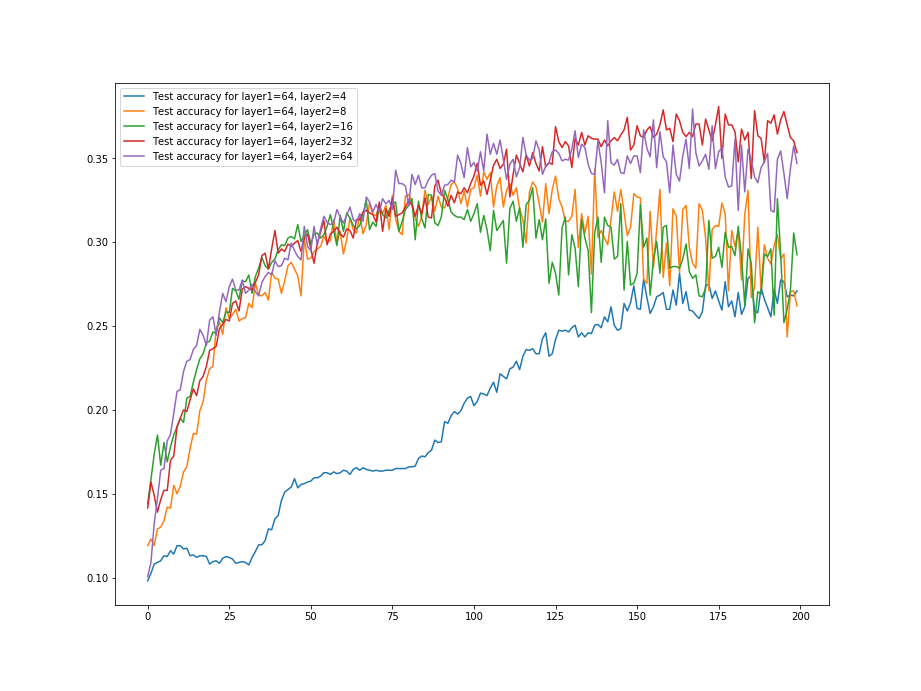
\includegraphics[width=1\linewidth]{assets/plots1/q2_4.png}
        \caption{Test accuracy for cnn}
    \end{subfigure}
    \caption{Plot of testing accuracy against epochs for different number of feature maps}
    \label{fig:2}
\end{figure}

From the results as shown in Figure \ref{fig:2_4}, having 32 feature maps in convolution layer 1 and 64 feature maps in convolution layer 2 resulted in the highest accuracy among all the others.


\subsection{Question 3}
\label{1q3}
\begin{quote}
Using the optimal number of filters found in part (2), train the network by:

a. Adding the momentum term with momentum $\gamma = 0.1$.

b. Using RMSProp algorithm for learning

c. Using Adam optimizer for learning

d. Adding dropout to the layers

Plot the training costs and test accuracies against epochs for each case.
\end{quote}

\begin{figure}[H]
    \begin{subfigure}{0.5\textwidth}
        \centering
        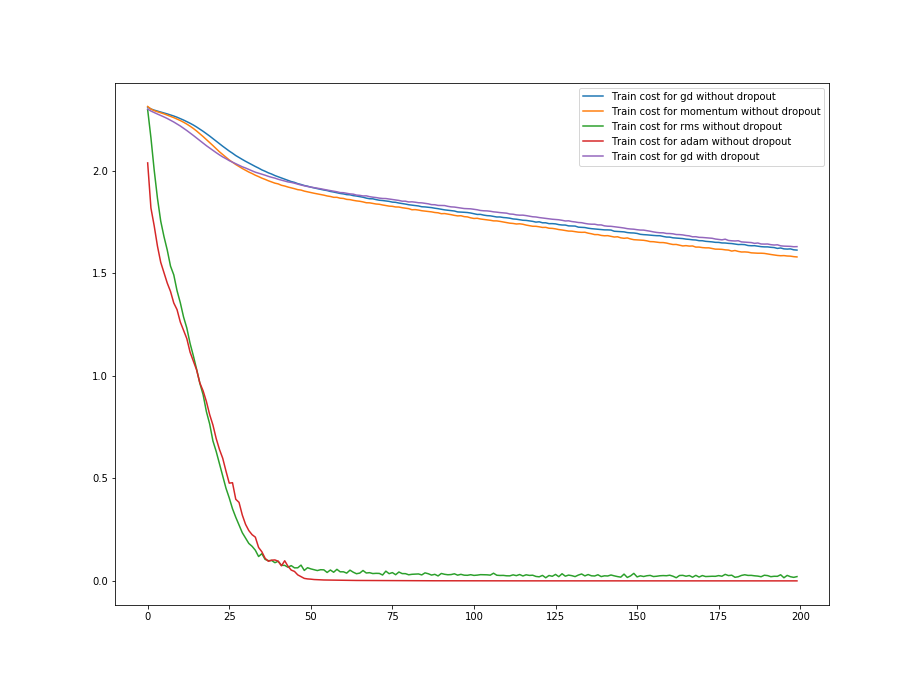
\includegraphics[width=1\linewidth]{assets/plots1/q3_1.png}
        \caption{Training cost for CNN}
        \label{fig:3_a}
    \end{subfigure}
    \begin{subfigure}{0.5\textwidth}
        \centering
        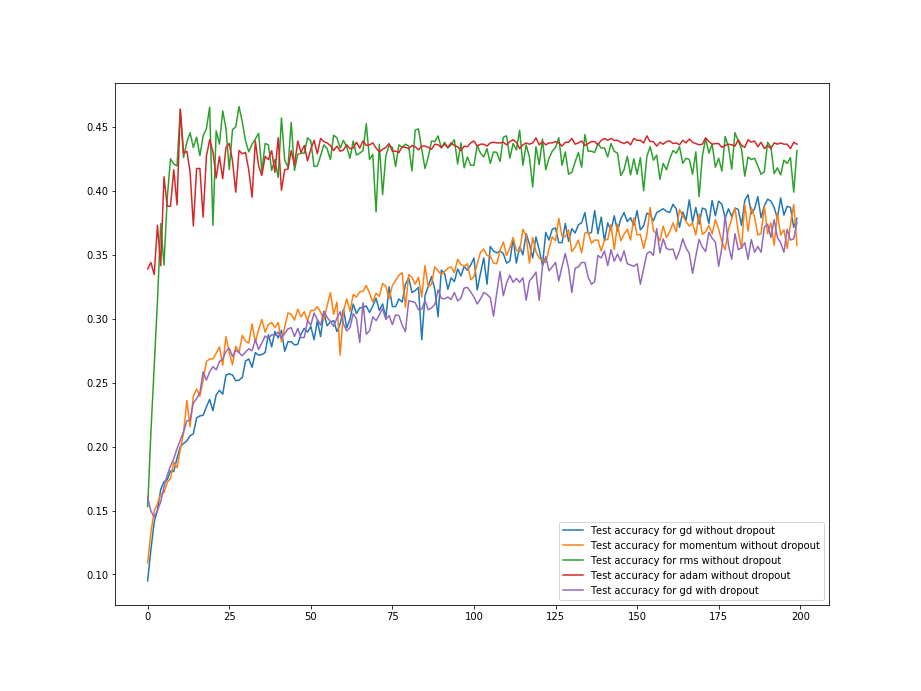
\includegraphics[width=1\linewidth]{assets/plots1/q3_2.png}
        \caption{Testing accuracy for CNN}
        \label{fig:3_b}
    \end{subfigure}
    \caption{Plot of training cost and testing accuracy against epochs for different optimizers}
    \label{fig:3}
\end{figure}

\subsection{Question 4}
\label{1q4}
\begin{quote}
Compare the accuracies of all the models from parts (1) - (3) and discuss their performances.
\end{quote}

For this experiment, we compared the performances against the original network without dropout. For network with momentum added, the accuracy is similar to the original network but its has a better learning rate as shown as the gradient being steeper. This is due to the fact that momentum causes the algorithm converges faster because oscillations are kept in one direction hence allowing a higher learning rate. Also, the RMSProp and Adam optimizers converges a lot faster in Figure \ref{fig:3_a} and has higher accuracy in Figure \ref{fig:3_a} than the other networks using other optimizers.

For the network using RMSProp, it has significantly better accuracy and performance compared to just adding momentum. It has a very high learning rate and it takes a larger step towards the minima. This is because it restricts the window of past gradients that are accumulated to be some fixed size. This ensures that learning continues to make progress even after many iterations of updates have been done. It uses an exponentially decaying average to discard the history from extreme past and this causes the algorithm to converge at a faster rate. 

The network using the Adam Optimizer has the best performance because it uses an adaptive learning rate method. Learning rates are stored for every parameter in the Adam Optimizer and it uses the squared gradients to scale the learning rate and the decaying average of the gradient instead of gradient itself. This resulted in high learning rate similar to when RMSProp is used and it has less fluctuations in the accuracy as reflected in Figure \ref{fig:3}. 